\documentclass{standalone}
\usepackage{tikz}
\usetikzlibrary{patterns, positioning}


\begin{document}
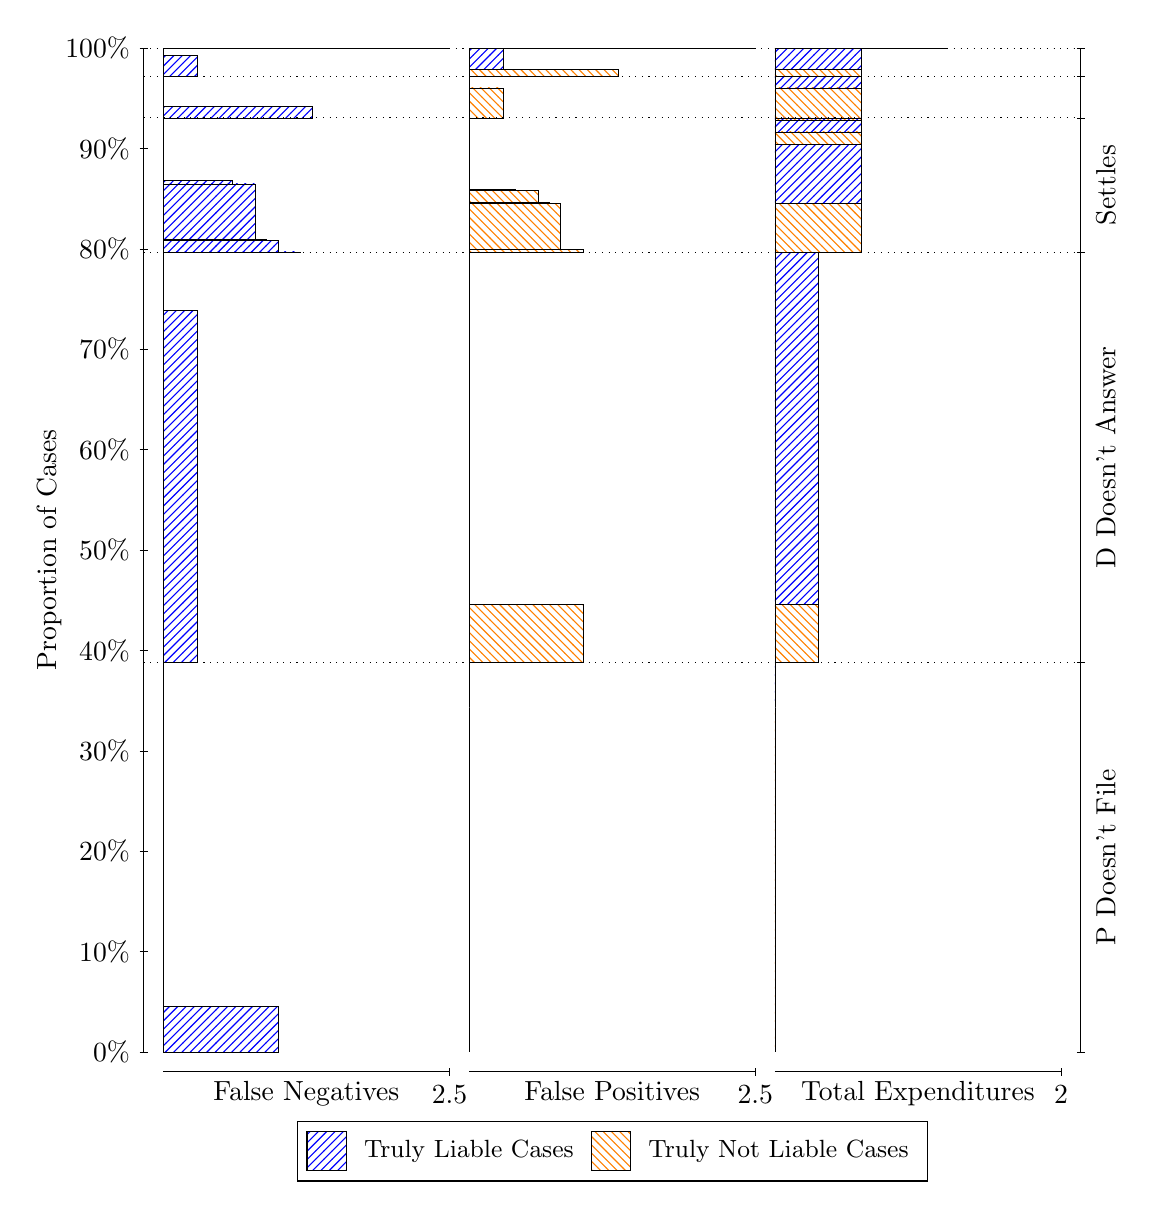
\begin{tikzpicture}
\draw[black, very thin] (1.5,1.75) -- (1.5,14.5);
\node[rotate=90, text=black, anchor=center] at (0.3, 8.125) {Proportion of Cases};
\draw[black, very thin] (1.45,1.75) -- (1.55,1.75);
\node[text=black, anchor=east] at (1.45, 1.75) {0\%};
\draw[black, very thin] (1.45,3.025) -- (1.55,3.025);
\node[text=black, anchor=east] at (1.45, 3.025) {10\%};
\draw[black, very thin] (1.45,4.3) -- (1.55,4.3);
\node[text=black, anchor=east] at (1.45, 4.3) {20\%};
\draw[black, very thin] (1.45,5.575) -- (1.55,5.575);
\node[text=black, anchor=east] at (1.45, 5.575) {30\%};
\draw[black, very thin] (1.45,6.85) -- (1.55,6.85);
\node[text=black, anchor=east] at (1.45, 6.85) {40\%};
\draw[black, very thin] (1.45,8.125) -- (1.55,8.125);
\node[text=black, anchor=east] at (1.45, 8.125) {50\%};
\draw[black, very thin] (1.45,9.4) -- (1.55,9.4);
\node[text=black, anchor=east] at (1.45, 9.4) {60\%};
\draw[black, very thin] (1.45,10.675) -- (1.55,10.675);
\node[text=black, anchor=east] at (1.45, 10.675) {70\%};
\draw[black, very thin] (1.45,11.95) -- (1.55,11.95);
\node[text=black, anchor=east] at (1.45, 11.95) {80\%};
\draw[black, very thin] (1.45,13.225) -- (1.55,13.225);
\node[text=black, anchor=east] at (1.45, 13.225) {90\%};
\draw[black, very thin] (1.45,14.5) -- (1.55,14.5);
\node[text=black, anchor=east] at (1.45, 14.5) {100\%};

\draw[black, very thin] (13.4,1.75) -- (13.4,14.5);
\draw[black, very thin] (13.35,1.75) -- (13.45,1.75);
\node[anchor=west] at (13.35, 1.75) {};
\draw[black, very thin] (13.35,6.6982) -- (13.45,6.6982);
\node[anchor=west] at (13.35, 6.6982) {};
\draw[black, very thin] (13.35,11.908) -- (13.45,11.908);
\node[anchor=west] at (13.35, 11.908) {};
\draw[black, very thin] (13.35,13.614) -- (13.45,13.614);
\node[anchor=west] at (13.35, 13.614) {};
\draw[black, very thin] (13.35,14.139) -- (13.45,14.139);
\node[anchor=west] at (13.35, 14.139) {};
\draw[black, very thin] (13.35,14.494) -- (13.45,14.494);
\node[anchor=west] at (13.35, 14.494) {};
\draw[black, very thin] (13.35,14.497) -- (13.45,14.497);
\node[anchor=west] at (13.35, 14.497) {};
\draw[black, very thin] (13.35,14.5) -- (13.45,14.5);
\node[anchor=west] at (13.35, 14.5) {};

\draw[black, very thin, pattern color=blue, pattern=north east lines] (1.75,1.75) rectangle (3.2033,2.3246);
\draw[black, very thin, pattern color=orange, pattern=north west lines] (1.75,2.3246) rectangle (1.75,6.6982);
\draw[black, very thin, pattern color=blue, pattern=north east lines] (1.75,6.6982) rectangle (2.186,11.169);
\draw[black, very thin, pattern color=orange, pattern=north west lines] (1.75,11.169) rectangle (1.75,11.908);
\draw[black, very thin, pattern color=blue, pattern=north east lines] (1.75,11.908) rectangle (3.494,11.91);
\draw[black, very thin, pattern color=blue, pattern=north east lines] (1.75,11.91) rectangle (3.2033,12.057);
\draw[black, very thin, pattern color=blue, pattern=north east lines] (1.75,12.057) rectangle (3.058,12.06);
\draw[black, very thin, pattern color=blue, pattern=north east lines] (1.75,12.06) rectangle (3.058,12.072);
\draw[black, very thin, pattern color=blue, pattern=north east lines] (1.75,12.072) rectangle (2.9127,12.775);
\draw[black, very thin, pattern color=blue, pattern=north east lines] (1.75,12.775) rectangle (2.622,12.822);
\draw[black, very thin, pattern color=orange, pattern=north west lines] (1.75,12.822) rectangle (1.75,13.614);
\draw[black, very thin, pattern color=blue, pattern=north east lines] (1.75,13.614) rectangle (3.6393,13.76);
\draw[black, very thin, pattern color=orange, pattern=north west lines] (1.75,13.76) rectangle (1.75,14.139);
\draw[black, very thin, pattern color=blue, pattern=north east lines] (1.75,14.139) rectangle (2.186,14.407);
\draw[black, very thin, pattern color=orange, pattern=north west lines] (1.75,14.407) rectangle (1.75,14.494);
\draw[black, very thin, pattern color=blue, pattern=north east lines] (1.75,14.494) rectangle (5.3833,14.495);
\draw[black, very thin, pattern color=orange, pattern=north west lines] (1.75,14.495) rectangle (1.75,14.497);
\draw[black, very thin, pattern color=orange, pattern=north west lines] (1.75,14.497) rectangle (1.75,14.499);
\draw[black, very thin, pattern color=blue, pattern=north east lines] (1.75,14.499) rectangle (1.75,14.5);
\draw[black, very thin, pattern color=orange, pattern=north west lines] (5.6333,1.75) rectangle (5.6333,6.1237);
\draw[black, very thin, pattern color=blue, pattern=north east lines] (5.6333,6.1237) rectangle (5.6333,6.6982);
\draw[black, very thin, pattern color=orange, pattern=north west lines] (5.6333,6.6982) rectangle (7.0867,7.4374);
\draw[black, very thin, pattern color=blue, pattern=north east lines] (5.6333,7.4374) rectangle (5.6333,11.908);
\draw[black, very thin, pattern color=orange, pattern=north west lines] (5.6333,11.908) rectangle (7.0867,11.945);
\draw[black, very thin, pattern color=orange, pattern=north west lines] (5.6333,11.945) rectangle (6.796,12.525);
\draw[black, very thin, pattern color=orange, pattern=north west lines] (5.6333,12.525) rectangle (6.6507,12.542);
\draw[black, very thin, pattern color=orange, pattern=north west lines] (5.6333,12.542) rectangle (6.5053,12.695);
\draw[black, very thin, pattern color=orange, pattern=north west lines] (5.6333,12.695) rectangle (6.2147,12.701);
\draw[black, very thin, pattern color=blue, pattern=north east lines] (5.6333,12.701) rectangle (5.6333,13.614);
\draw[black, very thin, pattern color=orange, pattern=north west lines] (5.6333,13.614) rectangle (6.0693,13.994);
\draw[black, very thin, pattern color=blue, pattern=north east lines] (5.6333,13.994) rectangle (5.6333,14.139);
\draw[black, very thin, pattern color=orange, pattern=north west lines] (5.6333,14.139) rectangle (7.5227,14.226);
\draw[black, very thin, pattern color=blue, pattern=north east lines] (5.6333,14.226) rectangle (6.0693,14.494);
\draw[black, very thin, pattern color=orange, pattern=north west lines] (5.6333,14.494) rectangle (5.6333,14.496);
\draw[black, very thin, pattern color=blue, pattern=north east lines] (5.6333,14.496) rectangle (5.6333,14.497);
\draw[black, very thin, pattern color=orange, pattern=north west lines] (5.6333,14.497) rectangle (9.2667,14.499);
\draw[black, very thin, pattern color=blue, pattern=north east lines] (5.6333,14.499) rectangle (7.8133,14.5);
\draw[black, very thin, pattern color=orange, pattern=north west lines] (9.5167,1.75) rectangle (9.5167,6.1237);
\draw[black, very thin, pattern color=blue, pattern=north east lines] (9.5167,6.1237) rectangle (9.5167,6.6982);
\draw[black, very thin, pattern color=orange, pattern=north west lines] (9.5167,6.6982) rectangle (10.062,7.4374);
\draw[black, very thin, pattern color=blue, pattern=north east lines] (9.5167,7.4374) rectangle (10.062,11.908);
\draw[black, very thin, pattern color=orange, pattern=north west lines] (9.5167,11.908) rectangle (10.607,12.525);
\draw[black, very thin, pattern color=blue, pattern=north east lines] (9.5167,12.525) rectangle (10.607,13.275);
\draw[black, very thin, pattern color=orange, pattern=north west lines] (9.5167,13.275) rectangle (10.607,13.436);
\draw[black, very thin, pattern color=blue, pattern=north east lines] (9.5167,13.436) rectangle (10.607,13.588);
\draw[black, very thin, pattern color=orange, pattern=north west lines] (9.5167,13.588) rectangle (10.607,13.603);
\draw[black, very thin, pattern color=blue, pattern=north east lines] (9.5167,13.603) rectangle (10.607,13.614);
\draw[black, very thin, pattern color=orange, pattern=north west lines] (9.5167,13.614) rectangle (10.607,13.994);
\draw[black, very thin, pattern color=blue, pattern=north east lines] (9.5167,13.994) rectangle (10.607,14.139);
\draw[black, very thin, pattern color=orange, pattern=north west lines] (9.5167,14.139) rectangle (10.607,14.226);
\draw[black, very thin, pattern color=blue, pattern=north east lines] (9.5167,14.226) rectangle (10.607,14.494);
\draw[black, very thin, pattern color=orange, pattern=north west lines] (9.5167,14.494) rectangle (11.697,14.496);
\draw[black, very thin, pattern color=blue, pattern=north east lines] (9.5167,14.496) rectangle (11.697,14.497);
\draw[black, very thin, pattern color=orange, pattern=north west lines] (9.5167,14.497) rectangle (11.697,14.499);
\draw[black, very thin, pattern color=blue, pattern=north east lines] (9.5167,14.499) rectangle (11.697,14.5);
\draw[black, dotted] (1.5,6.6982) -- (13.4,6.6982);
\draw[black, dotted] (1.5,11.908) -- (13.4,11.908);
\draw[black, dotted] (1.5,13.614) -- (13.4,13.614);
\draw[black, dotted] (1.5,14.139) -- (13.4,14.139);
\draw[black, dotted] (1.5,14.494) -- (13.4,14.494);
\draw[black, dotted] (1.5,14.497) -- (13.4,14.497);
\draw[black, very thin] (1.75,1.5) -- (5.3833,1.5);
\node[text=black, anchor=north] at (3.5667, 1.5) {False Negatives};
\draw[black, very thin] (5.3833,1.45) -- (5.3833,1.55);
\node[text=black, anchor=north] at (5.3833, 1.45) {2.5};

\draw[black, very thin] (5.6333,1.5) -- (9.2667,1.5);
\node[text=black, anchor=north] at (7.45, 1.5) {False Positives};
\draw[black, very thin] (9.2667,1.45) -- (9.2667,1.55);
\node[text=black, anchor=north] at (9.2667, 1.45) {2.5};

\draw[black, very thin] (9.5167,1.5) -- (13.15,1.5);
\node[text=black, anchor=north] at (11.333, 1.5) {Total Expenditures};
\draw[black, very thin] (13.15,1.45) -- (13.15,1.55);
\node[text=black, anchor=north] at (13.15, 1.45) {2};

\node[text=black, centered, rotate=90] at (13.72, 4.2241) {P Doesn't File};
\node[text=black, centered, rotate=90] at (13.72, 9.3031) {D Doesn't Answer};
\node[text=black, centered, rotate=90] at (13.72, 12.761) {Settles};





\draw (7.449999999999999,1.5) node[draw=none] (baseCoordinate) {};
\begin{scope}[align=center]
        \matrix[scale=0.5, draw=black, below=0.5cm of baseCoordinate, nodes={draw}, column sep=0.1cm]{
            \node[rectangle, draw, minimum width=0.5cm, minimum height=0.5cm, pattern color=blue, pattern=north east lines] {}; &
            \node[draw=none, font=\small, text=black] (B) {Truly Liable Cases}; &
            \node[rectangle, draw, minimum width=0.5cm, minimum height=0.5cm, pattern color=orange, pattern=north west lines] {}; &
            \node[draw=none, font=\small, text=black] (B) {Truly Not Liable Cases}; \\
            };
\end{scope}

\end{tikzpicture}
\end{document}